\documentclass[12pt]{article}
%\usepackage[utf8]{inputenc}
\usepackage{indentfirst}
\usepackage{float}
\usepackage{array}
\usepackage{listings}
\usepackage{csquotes}
\usepackage{url}
\urlstyle{tt}
\usepackage{enumitem, amsmath, amssymb, amsfonts, latexsym, mathrsfs}
\usepackage{graphicx}
\usepackage{subfig}
\usepackage{multicol}
\usepackage{booktabs}
\usepackage{ragged2e}

\usepackage{multicol}
\setlength{\columnseprule}{1pt}
\def\columnseprulecolor{\color{black}}

\usepackage{svg}
\usepackage{xcolor}

\usepackage[spanish]{babel}
\usepackage[utf8]{inputenc}
\usepackage[backend=biber]{biblatex}
\bibliography{referencias}

\date{}
% Comand para keywords
\providecommand{\keywords}[1]
{
  \small	
  \textbf{\textit{Keywords---}} #1
}

% Tipografía
%\usepackage{helvet}
%\renewcommand{\familydefault}{\sfdefault}
%\usepackage[sfdefault]{Chivo}
%\usepackage{comment}

\usepackage[sfdefault]{atkinson} %% Option 'sfdefault' if the base
%% font of the document is to be sans serif.
\usepackage{fontspec}
\renewcommand{\familydefault}{\sfdefault}

\urlstyle{same}
% \tolerance=9999
% \emergencystretch=10pt
\hyphenpenalty=10000
\sloppy
% \exhyphenpenalty=100

\renewcommand{\figurename}{\textbf{Figura.}}
\renewcommand\spanishtablename{Tabla.}

% Interlineado
\usepackage{setspace}
\spacing{1.15}

% Márgenes
\usepackage[a4paper]{geometry}
\geometry{top=2.5cm, bottom=2.5cm, left=2cm, right=2cm}

% Número de página
\usepackage{fancyhdr}
\pagestyle{fancy}
\rhead[]{}
\lhead[]{}
\renewcommand{\headrulewidth}{0pt}
\rfoot[]{\thepage}
\cfoot[]{}

\usepackage[breaklinks]{hyperref}
% Setup de hiperenlaces
\hypersetup{
    colorlinks=true,
    linkcolor=blue,
    filecolor=magenta,      
    urlcolor=cyan,
    pdftitle={Arquitectura de las consolas de videojuegos},
    pdfpagemode=FullScreen,
    citecolor = green
    }
\usepackage[norule]{footmisc}

%_____________________________________________________________________________
%_____________________________________________________________________________
%_____________________________________________________________________________
%_____________________________________________________________________________
\hbadness=50000
\usepackage{microtype}
\begin{document}
\nocite{atkinson}
% PORTADA
        \begin{center}
             
         
        \hrule
        \vspace{1cm}
        %{\bfseries\Large UNIVERSIDAT JAUME I \par}
        \vspace{1cm}
        {\bfseries\huge Apuntes de Consolas y Dispositivos de Videojuegos \par}
        \vspace{2cm}

        \begin{figure}[H]
            \centering
            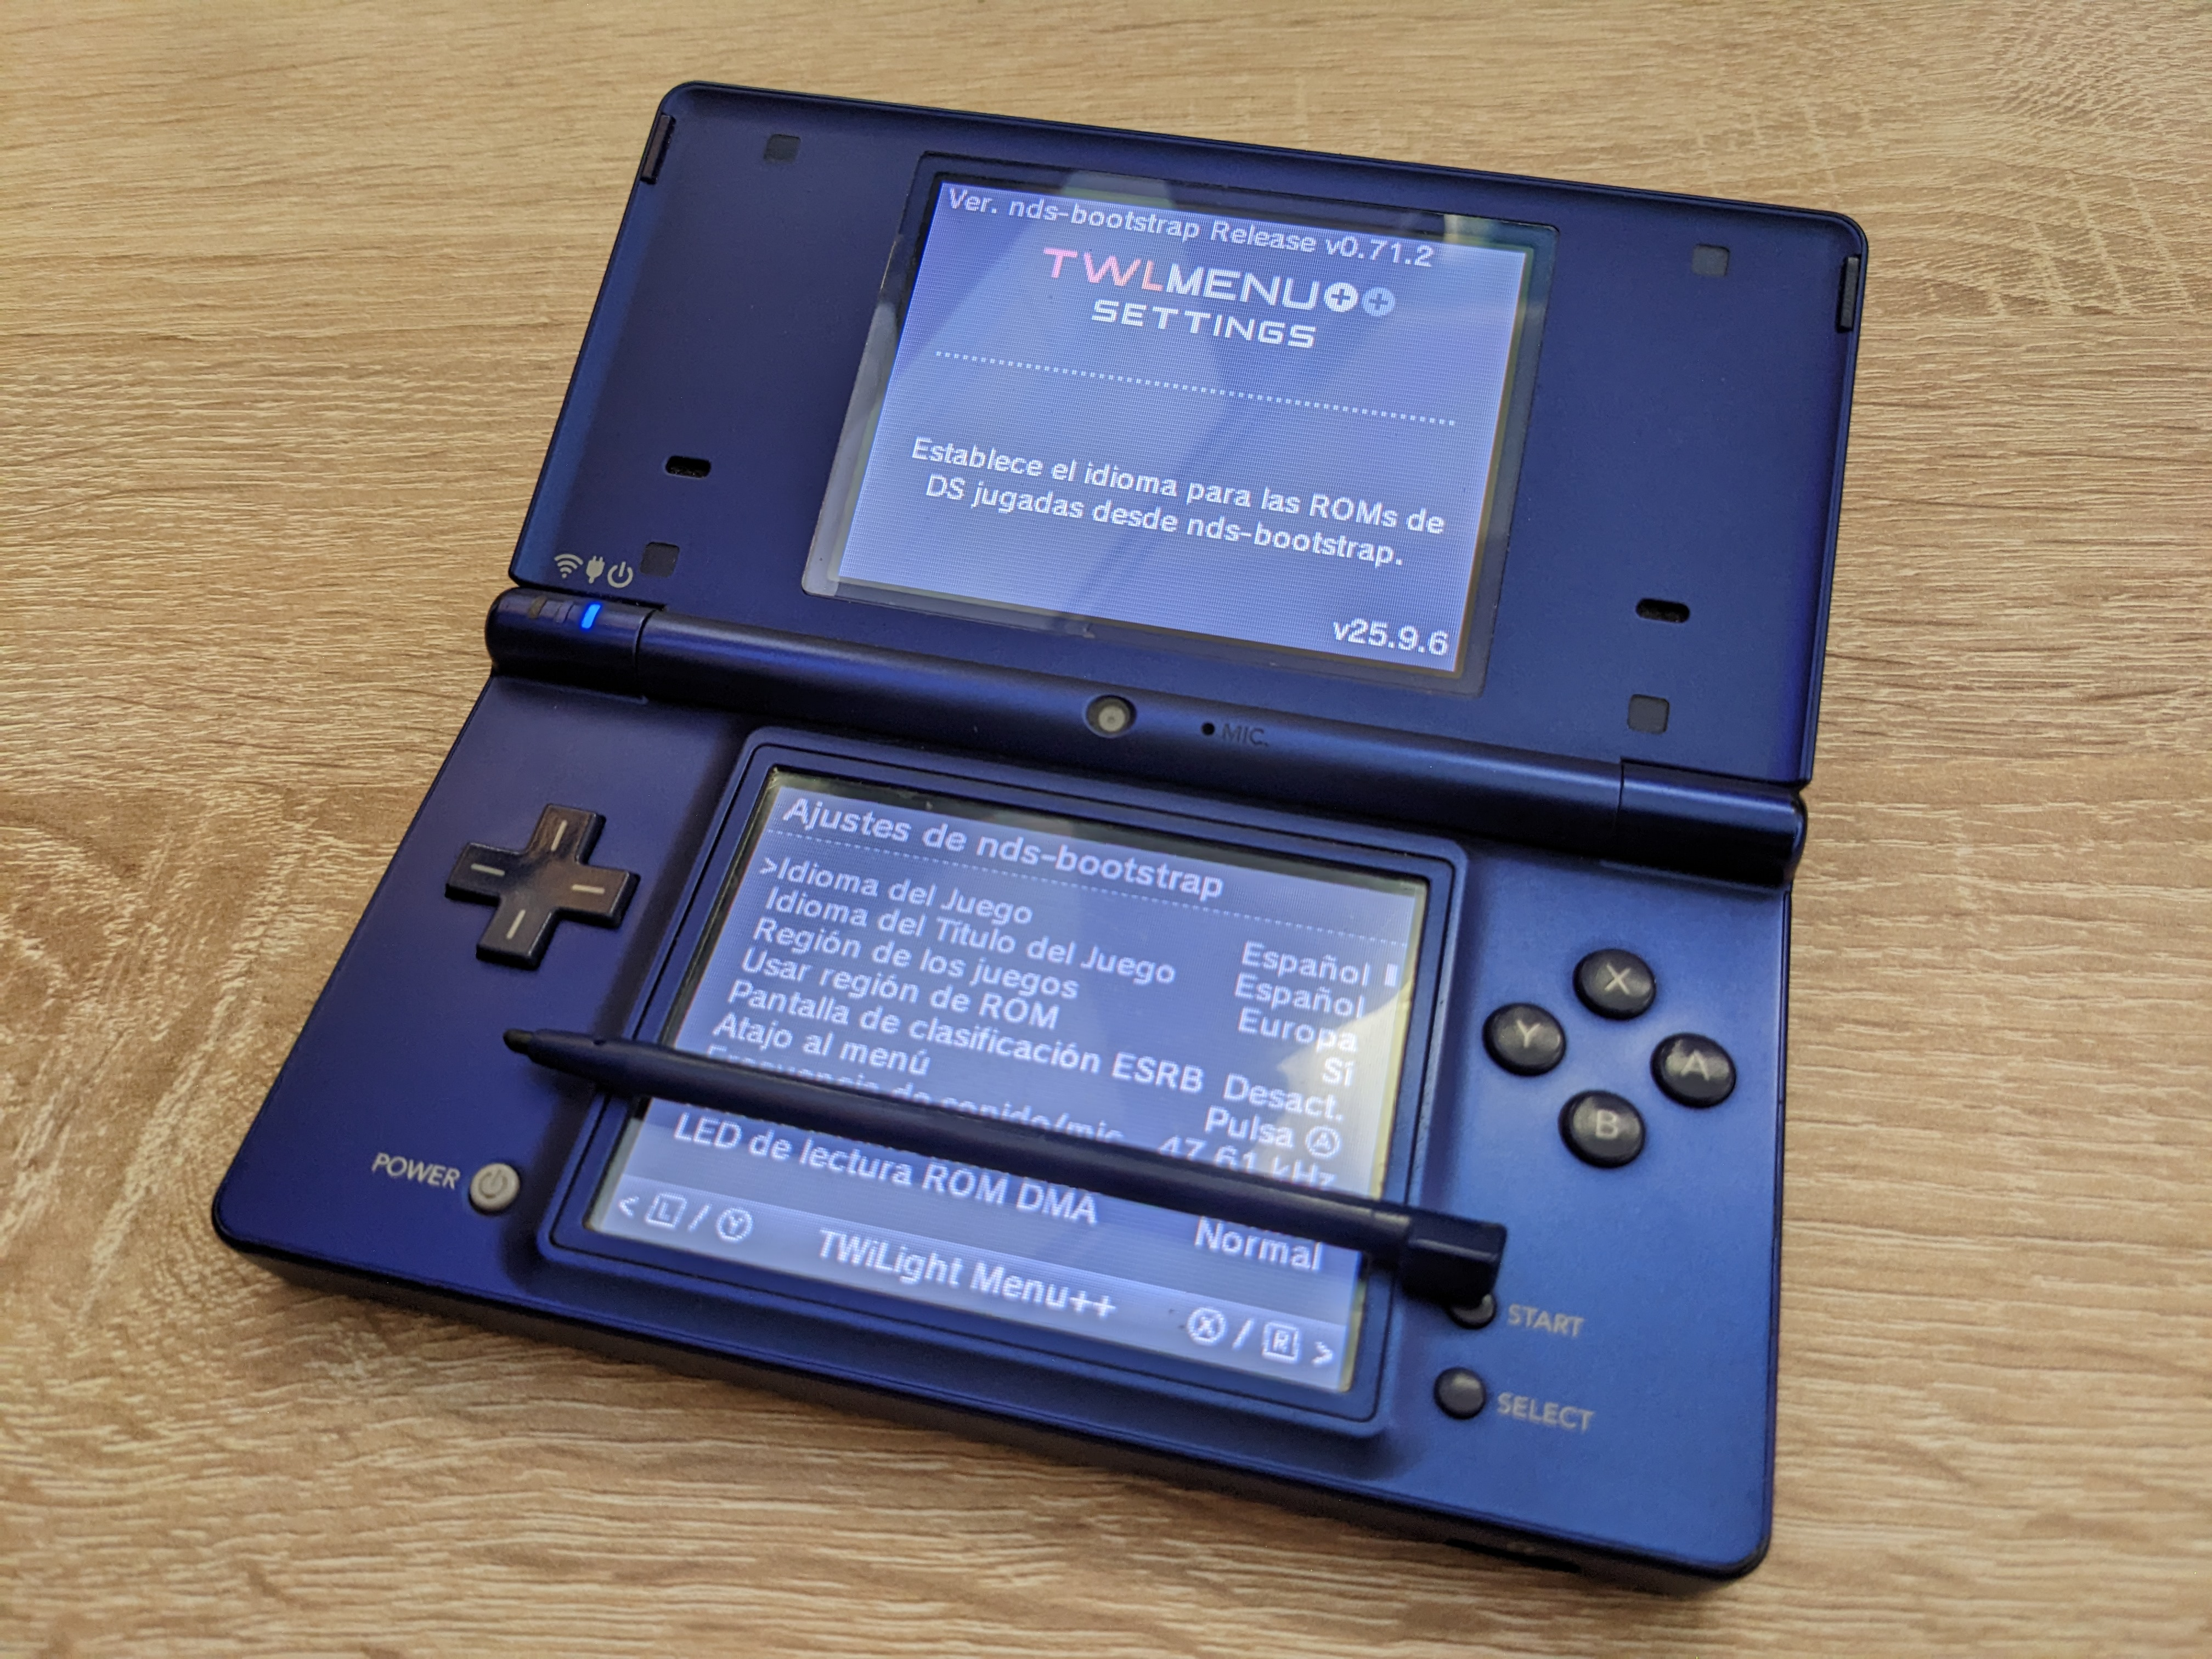
\includegraphics[width=\textwidth]{PXL_20230917_103129958.NIGHT.jpg}
            \caption{Nintendo DSi con Homebrew y emulador de NDS}
            \label{fig:dsi}
        \end{figure}
        
        {\large 
        Jesús Jimenez Montero \\
        \par}
        \vspace{1cm}
        \hrule
        \vspace{1cm}

        {\large 
        \textit{Versión 1: Boole; expresiones y tablas de verdad, mapas de Karnaugh\\
        Fecha: 18/09/2023}
        \par}
        \end{center}

% ÍNDICE
%\renewcommand{\tableofcontents}{Indice general}
\newpage
\renewcommand{\contentsname}{Tabla de contenidos}
\setcounter{secnumdepth}{5}
\tableofcontents
\setcounter{tocdepth}{4}

\newpage
%-----------------------------------------------------------------
%-----------------------------------------------------------------
% Tabla de figuras
\newpage
\renewcommand{\listfigurename}{Lista de figuras}
\thispagestyle{empty}
\listoffigures
\newpage

\renewcommand{\listtablename}{Lista de tablas}
\listoftables
\newpage

%-----------------------------------------------------------------
%-----------------------------------------------------------------

\section{El álgebra de Boole}

    \subsection{Definición del algebra de Boole \cite{floyd_fundamentos_2006} \cite{logic_gate} \cite{puerta_logica}}
        El álgebra de Boole es basicamente las matématicas que se usan en computación, necesarias para analizar los circuitos lógicos. 

        Para realizar esta álgebra se usan varios términos: variable, que referencia a una magnitud que se resume en los valores 0 y 1 y los complementos, que son los inversos de una variable, representados con una barra ($A \rightarrow \overline{A}$). 

        Las puertas lógicas son circuitos que realizan operaciones lógicas determinadas: 
        
            \subsubsection{\textbf{Puerta lógica NOT}}
            
            Negación booleana, $A$ pasa a ser no $A$, es decir, $\overline{A}$.

                \begin{multicols}{2}

\begin{table}[H]
    \centering
                        \begin{tabular}{|c|c|}
                            $A$ & $\overline{A}$ \\
                            \hline
                            0 & 1 \\
                            1 & 0
                        \end{tabular}
    \caption{Tabla de verdad de NOT}
    \label{tab:not}
\end{table}
                           
                    \columnbreak
                    \newpage
                    \begin{figure}[H]
                        \centering
                        \includesvg{NOT_ANSI_Labelled.svg}
                        \caption{Diagrama de puerta lógica \textit{NOT} \cite{logic_gate}}
                        \label{fig:not}
                    \end{figure}
                \end{multicols}
                
            \subsubsection{\textbf{Puerta lógica OR}}
            
            Suma booleana $A + B$. La suma es igual a 1 si alguno de los literales es 1; y es igual a 0 si todos los literales son 0.

            \begin{multicols}{2}

\begin{table}[H]
    \centering
                \begin{tabular}{|c c|c}
                    $A$ & $B$ & $A + B$ \\
                    \hline
                    0 & 0 & 0 \\
                    0 & 1 & 1 \\
                    1 & 0 & 1 \\
                    1 & 1 & 1
                \end{tabular}
    \caption{Tabla de verdad de OR}
    \label{tab:my_label}
\end{table}

                                

                \columnbreak
                \newpage
                \begin{figure}[H]
                    \centering
                    \includesvg{OR_ANSI_Labelled.svg}
                    \caption{Diagrama de puerta lógica \textit{OR} \cite{logic_gate}}
                    \label{fig:or}
                \end{figure}

            \end{multicols}
            
            \subsubsection{\textbf{Puerta lógica AND}}
            
            Multiplicación booleana $AB$. Solo da como resultado un 1 cuando todas las variables son 1, y en el resto, 0.
            
            \begin{multicols}{2}
\begin{table}[H]
    \centering
                \begin{tabular}{|c c|c}
                    $A$ & $B$ & $AB$ \\
                    \hline
                    0 & 0 & 0 \\
                    0 & 1 & 0 \\
                    1 & 0 & 0 \\
                    1 & 1 & 1
                \end{tabular}
    \caption{Tabla de verdad de AND}
    \label{tab:my_label}
\end{table}


                \columnbreak
                \newpage
                \begin{figure}[H]
                    \centering
                    \includesvg{AND_ANSI_Labelled.svg}
                    \caption{Diagrama de puerta lógica \textit{AND} \cite{logic_gate}}
                    \label{fig:and}
                \end{figure}
            \end{multicols}

    \newpage
    \subsection{Conversión de tabla de verdad a expresión como suma de productos \cite{floyd_fundamentos_2006}}
        Usando tablas de verdad, se pueden crear expresiones:

            \begin{table}[H]
            \centering
            \resizebox{.35\textwidth}{!}{%
            \begin{tabular}{@{}rrrrl@{}}
            \toprule
            \multicolumn{1}{l}{} & \multicolumn{1}{l}{} & \multicolumn{1}{l}{} & \multicolumn{1}{l}{Salida} & Término \\ \midrule
            \multicolumn{1}{l}{A} & \multicolumn{1}{l}{B} & \multicolumn{1}{l}{C} & \multicolumn{1}{l}{F(ABC)} &  \\
            0 & 0 & 0 & 1 & $\overline{A}\overline{B}\overline{C}$ \\
            0 & 0 & 1 & 0 &  \\
            0 & 1 & 0 & 1 & $\overline{A}B\overline{C}$ \\
            0 & 1 & 1 & 1 & $\overline{A}BC$ \\
            1 & 0 & 0 & 1 & $A\overline{B}\overline{C}$ \\
            1 & 0 & 1 & 0 & $A\overline{B}C$ \\
            1 & 1 & 0 & 1 & $AB\overline{C}$ \\
            1 & 1 & 1 & 0 & $ABC$ \\ \bottomrule
            \end{tabular}
            }
            \caption{Tabla de verdad de la ecuación propuesta}
            \label{tab:verdad}
            \end{table}
            Como ejemplo, se introducen números aleatorios en la columna de salida F(ABC), se puede obtener una expresión, escribiendo las variables como \textit{NOT} cuando son 0 y sin \textit{NOT} cuando son 1. 
            
            Resultando en esta ecuación:
            
            $F(A,B,C) = \overline{A}\overline{B}\overline{C} + \overline{A}B\overline{C} + \overline{A}BC + A\overline{B}\overline{C} + A\overline{B}C + AB\overline{C} + ABC$
        \newpage
        \subsection{Simplificación de funciones lógicas con mapas de Karnaugh \cite{video_karnaugh}}
            Para simplificar ecuaciones en forma estándar, se pueden usar mapas de Karnaugh. Usando la ecuación del punto anterior, se simplifica de tal manera:

                Se introducen los términos de la anterior tabla donde corresponden. Por ejemplo, si $A$ = 0, $B$ = 1, y $C$ = 0; se introduce en la columna donde $AB$ son 01 y $C$ es 0. Y así hasta completar la tabla.
                % Please add the following required packages to your document preamble:
                % \usepackage{graphicx}
                % \usepackage[table,xcdraw]{xcolor}
                % If you use beamer only pass "xcolor=table" option, i.e. \documentclass[xcolor=table]{beamer}
                \begin{table}[H]
                \centering
                \resizebox{.35\textwidth}{!}{%
                \begin{tabular}{lllll}
                \hline
                AB/C & 00                       & 01                           & 11                       & 10                       \\ \hline
                0    & {\color[HTML]{4A86E8} 1} & {\color[HTML]{4A86E8} 1 \color[HTML]{000000} / \color[HTML]{FF9900} 1} & {\color[HTML]{4A86E8} 1} & {\color[HTML]{4A86E8} 1} \\
                1    & 0                        & {\color[HTML]{FF9900} 1}     & 0                        & 0                        \\ \hline
                \end{tabular}%
                }
                \caption{Mapa de Karnaugh de la tabla: \ref{tab:verdad} }
                \end{table}

                El resultado de la simplificación es: $\overline{C} + \overline{A}B$. 
                
                Siendo así debido a que el concepto principal de la simplificación con mapas de Karnaugh se basa en buscar variables que no cambien. 
                
                En el grupo de unos azules, como $C$ se mantiene constante, se simplifica a solo $C$ y se niega debido a que su \textit{output} es 0 en la fila donde se encuentra el grupo de unos azules.
                
                Y en el caso del grupo de los unos naranjas, las variables que no varían son $A$ y $B$, se descarta $C$ y se niega $A$ debido a que cambia su \textit{output} entre 0 y 1. 
    \newpage

\section{Puertas lógicas básicas}
    \subsection{NOT}
        \subsubsection{Tabla de verdad}
        \subsubsection{Esquema exterior del circuito}
        \subsubsection{Esquema interior del circuito}
        \subsubsection{Implmenetación interna con código HDL}
        \subsubsection{Test de funcionamiento}
    \newpage
    \subsection{AND}
        \subsubsection{Tabla de verdad}
        \subsubsection{Esquema exterior del circuito}
        \subsubsection{Esquema interior del circuito}
        \subsubsection{Implmenetación interna con código HDL}
        \subsubsection{Test de funcionamiento}      
    \newpage  
    \subsection{OR}
        \subsubsection{Tabla de verdad}
        \subsubsection{Esquema exterior del circuito}
        \subsubsection{Esquema interior del circuito}
        \subsubsection{Implmenetación interna con código HDL}
        \subsubsection{Test de funcionamiento}
    \newpage
    \subsection{XOR}
        El resultado es 0 si todos los términos son iguales y 1 si cualquier termino es diferente.
        $F(A,B) = Xor(A,B)$
        \subsubsection{Tabla de verdad}
        \subsubsection{Esquema exterior del circuito}
        \subsubsection{Esquema interior del circuito}
        \subsubsection{Implmenetación interna con código HDL}
        \subsubsection{Test de funcionamiento}
    \newpage
    \subsection{MUX}
        \subsubsection{Tabla de verdad}
        \subsubsection{Esquema exterior del circuito}
        \subsubsection{Esquema interior del circuito}
        \subsubsection{Implmenetación interna con código HDL}
        \subsubsection{Test de funcionamiento}
    \newpage
    \subsection{DMUX}
        \subsubsection{Tabla de verdad}
        \subsubsection{Esquema exterior del circuito}
        \subsubsection{Esquema interior del circuito}
        \subsubsection{Implmenetación interna con código HDL}
        \subsubsection{Test de funcionamiento}
    \newpage
    \subsection{NOT16}
        \subsubsection{Tabla de verdad}
        \subsubsection{Esquema exterior del circuito}
        \subsubsection{Esquema interior del circuito}
        \subsubsection{Implmenetación interna con código HDL}
        \subsubsection{Test de funcionamiento}
    \newpage
    \subsection{OR16}
        \subsubsection{Tabla de verdad}
        \subsubsection{Esquema exterior del circuito}
        \subsubsection{Esquema interior del circuito}
        \subsubsection{Implmenetación interna con código HDL}
        \subsubsection{Test de funcionamiento}
    \newpage
    \subsection{MUX16}
        \subsubsection{Tabla de verdad}
        \subsubsection{Esquema exterior del circuito}
        \subsubsection{Esquema interior del circuito}
        \subsubsection{Implmenetación interna con código HDL}
        \subsubsection{Test de funcionamiento}
    \newpage

\printbibliography[heading=bibintoc]
\end{document}
